\chapter{Testy}
\thispagestyle{chapterBeginStyle}

\section{15}
    \subsection{Wprowadzenie}
        Piętnastka (fr. taquin), znana również w Polsce o nazwie \textit{przesuwanka}, w zapisie często podawana przy pomocy liczbowego
        odpowiednika (15) jest grą w formie specyficznej
        układanki, której powstanie datuje się na koniec XIX wieku. Składa się ona z 
        15 klocków oraz ramki, pierwotnie drewnianej. Ramka zaprojektowana została specjalnie z myślą
        o pozostawieniu jednego wolnego miejsca, aby móc w łatwy sposób przesuwać klocki sąsiadujące z miejscem 
        pustym. Celem gry jest ułożenie klocków w określony sposób, najcześciej w porządku rosnącym czytając 
        od lewej do prawej rzędami, z określonego stanu początkowego. Częstym zabiegiem stosowanym przez 
        twórców ów układanki jest konwersja liczb na części obrazka, aby zachęcić do gry młodszych odbiorców.

        \begin{figure}[H]
            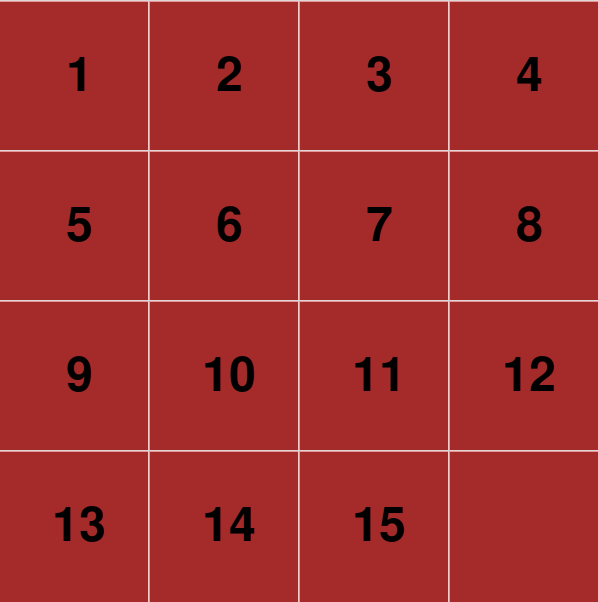
\includegraphics[scale=0.5]{15_ułożona}
            \centering
            \caption{Wygląd układanki piętnastki wygenerowany przy pomocy zaimplementowanej w ramach pracy warstwy graficznej}
        \end{figure}

        \begin{figure}[H]
            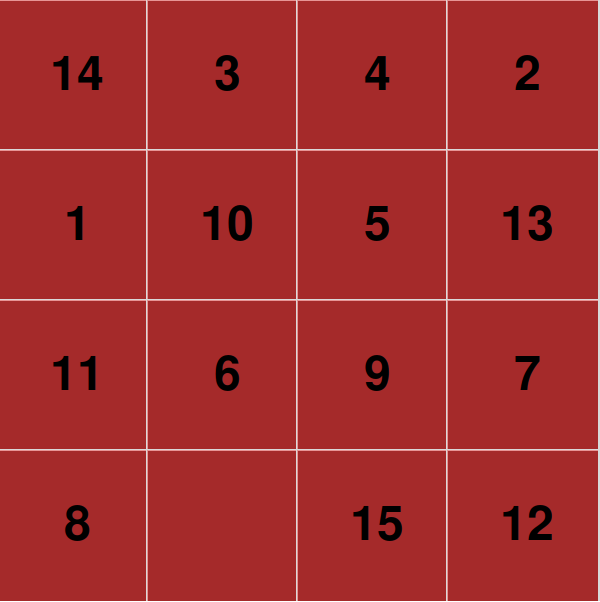
\includegraphics[scale=0.5]{15_losowe}
            \centering
            \caption{Losowa rozwiązywalna permutacja układanki}
        \end{figure}

        \begin{figure}[H]
            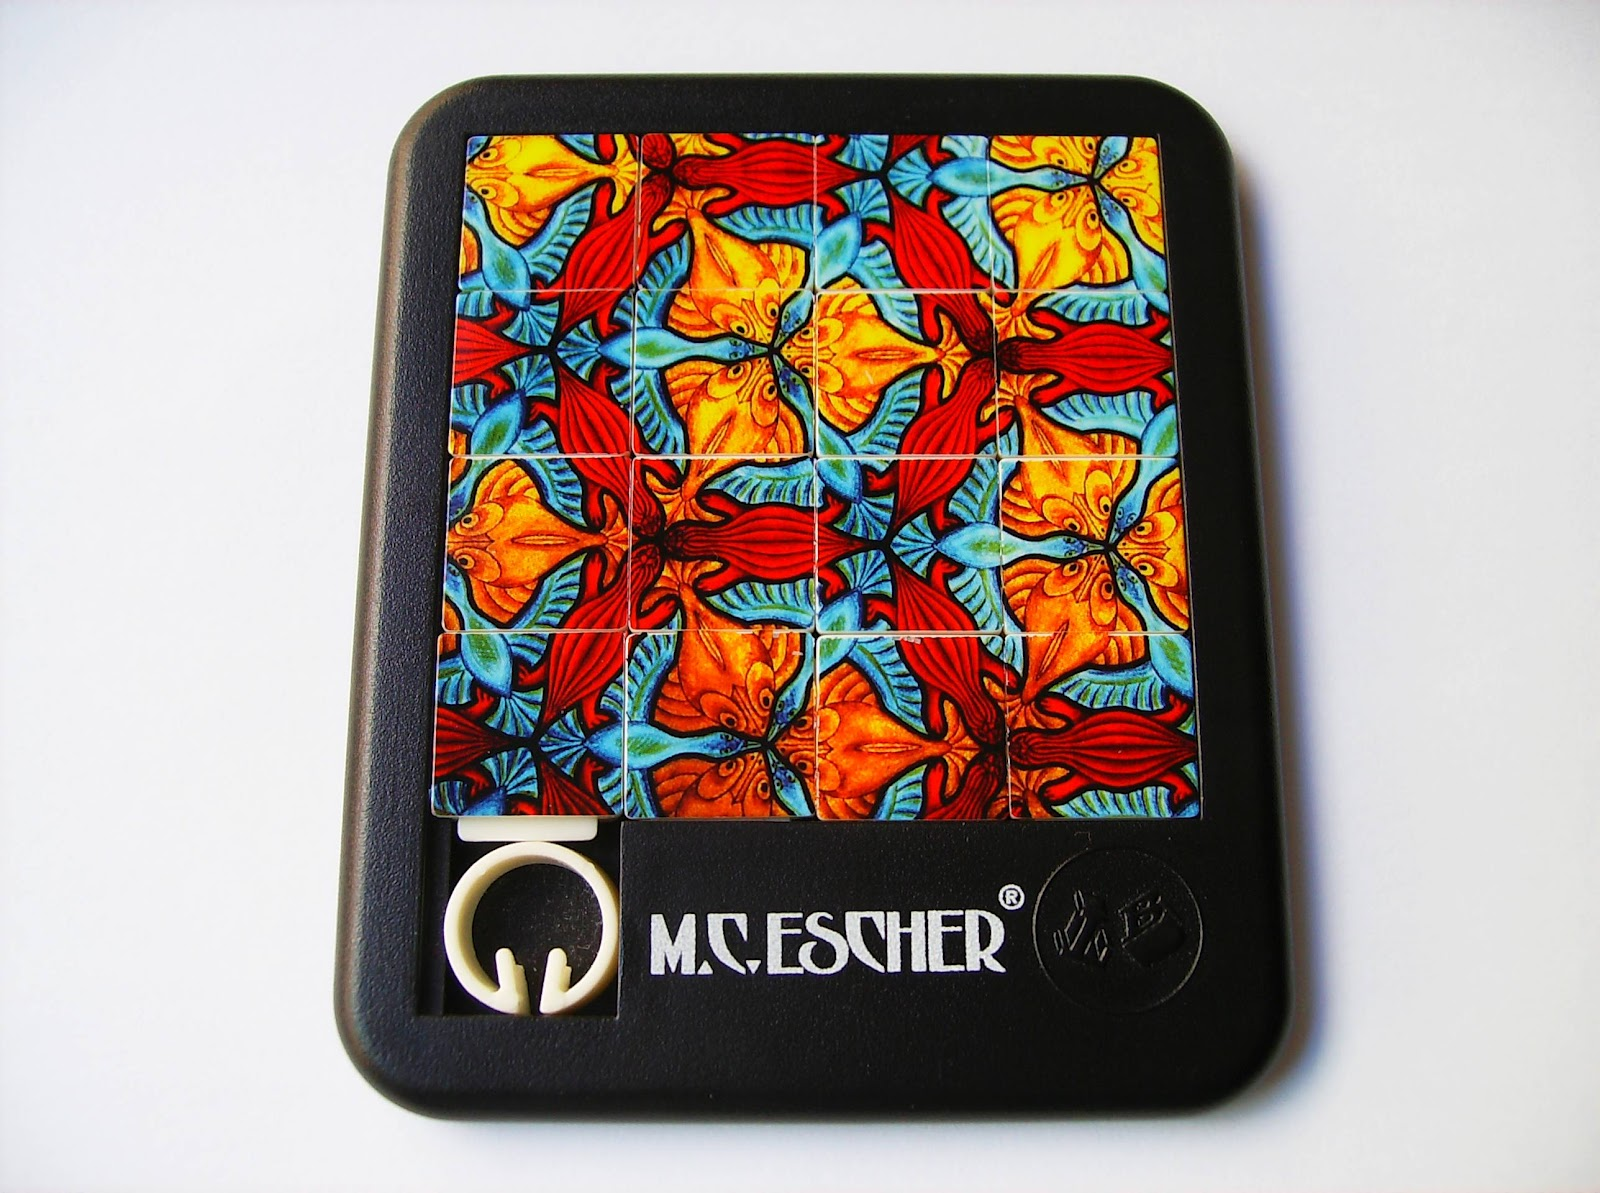
\includegraphics[scale=0.15]{15_obrazkowa}
            \centering
            \caption{Piętnastka w formie obrazkowej. Źródło: \url{http://mypuzzlecollection.blogspot.com/2012/08/mc-escher-birds-fish-and-turtles.html}}
        \end{figure}

    \subsection{Teoria}
        W 1878 roku amerykański wynalazca gier i zagadek (między innymi zagadek szachowych) \textbf{Samuel Loyd} ze względu na swój fach 
        nie przeszedł obojętnie koło piętnastki proponując ułożenie układu rosnącego z pozycji, która 
        od początkowej różniła się pozycjami jedynie dwóch klocków numerowanych odpowiednio 14 i 15 \cite{FifteenLoydProblem}.
        Problem ów stał się na tyle popularny, iż została wyznaczona nagroda 1000 dolarów dla osoby, której udałoby się 
        znaleźć prawidłowe rozwiązanie przygotowanego przez Pana Samuela problemu.

        Niemożliwość ułożenia problemu przez bardzo długi czas doprowadziła do pierwszych poważniejszych rozważań 
        nad z pozoru trywialną łamigówką. Efektem prac matematyków było parę zaskakujących wniosków, które ostatecznie doprowadziły 
        do udowodnienia, iż wyżej przedstawiona łamigłówka jest nierozwiązywalna.
        \begin{lemma}
            Nie wszystkie ustawienia początkowe piętnastki są możliwe do rozwiązania.\cite{Fifteen}
        \end{lemma}
        Wynika to z faktu, iż rozwiązywalne są jedynie rozwiązanie oo parzystej liczbie inwersji. Zagadka Pana Lyod'a jest 
        ustawieniem nieparzystym jeśli chodzi o inwersje. Prowadzi to do następującego wniosku:
        \begin{corollary}
            Istnieje $\frac{16!}{2}=10 461 394 944 000$ rozwiązywalnych ustawień. 
        \end{corollary}
        Dodatkową ciekawostką istotną z perspektywy wykonywanych testów jest minimalna liczba posunięć, którą należy wykonać, 
        aby z rozwiązywalnego stanu osiągnąć wcześniej wyznaczony cel. Mianem \textbf{boskiej liczby} w odniesieniu do przesuwanki
        określą się największą liczbę posunięć, którą trzeba osiągnąć, aby rozwiązać najtrudniejsze ułożeniem początkowe. Przy pomocy matematyki 
        naukowcy odnaleźli najtrudniejsze ustawienia oraz obliczyli ów liczbę, co zaprezentowano w następującym lemacie:
        \begin{lemma}
            \textbf{Boska liczba} dla 15-elementowej przesuwanki wynosi \textbf{80}. \cite{80Moves}
        \end{lemma}
        Oznacza to, iż maksymalna liczba kroków algorytmu w żadnym wypadku nie powinna przekroczyć liczby 80.

        W trakcie poniżej opisanego testu sprawdzono plany przesuwania odpowiednich klocków, aby w jak najmniejszej możliwej liczbie ruchów
        otrzymać odpowiedni stan końcowy, przy okazji sprawdzono osiągnięcia czasowe jak i porównano otrzymane wyniki z popularnymi herustykiami 
        spersonalizowanymi pod rozwiązywanie ów układanki.

    \subsection{Przykład}
        Na podstawie następującego przykładu zostanie przedstawiony schemat rozwiązywania układanki przez algorytm:
        \begin{figure}[H]
            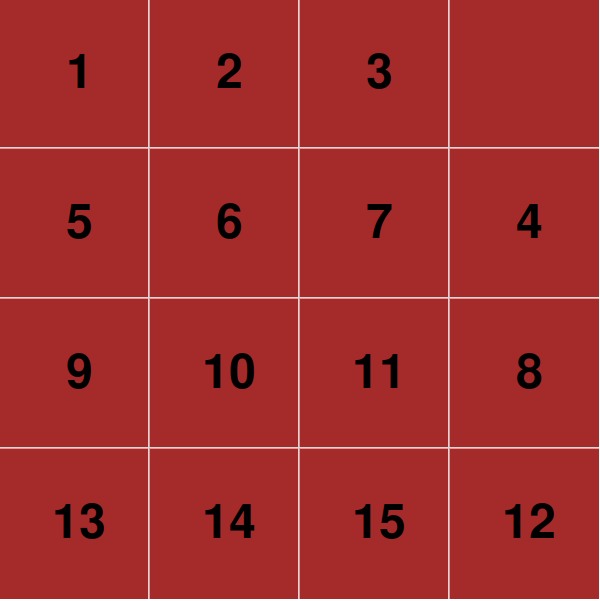
\includegraphics[scale=0.5]{15_przyklad}
            \centering
            \caption{Przykładowe startowe ułożenie przesuwanki}
        \end{figure}
        Algorytm buduje graf na podstawie jedynej zdefiniowanej w problemie akcji: przesuwania klocka. Robi to aż do momentu, gdy kafelki nie 
        będą ułożone w wczesniej zdefiniowanej kolejności. Dla zdefiniowanego powyżej przykładu w pierwszym kroku algorytm ma jedynie dwie możliwości 
        akcji aktywnych: zamiana klocka pustego z klockiem o numerze 3 lub klockiem o numerze 4. Na tej podstawie generuje kolejny poziom stanów. 
        Dla załączonego przykładu optymalnym rozwiązaniem jest odpowiednio zamiana pustego kafelka z kafelkami: 4,8,12, co zostało poprawnie 
        wyznaczone przez GRAPHPLAN. Poniżej przedstawiono zbiory akcji przeanalizowane przez algorytm w danym kroku jak i uproszczony graf planujący.

        \begin{figure}[H]
            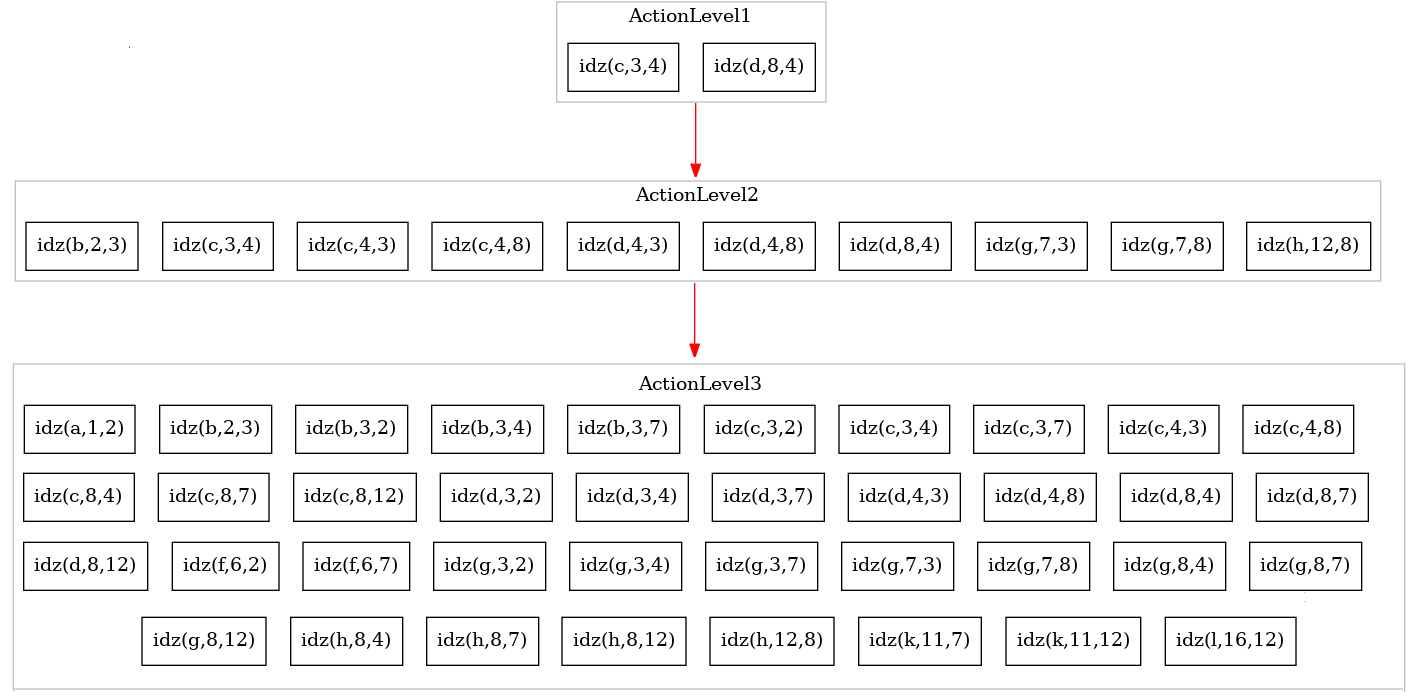
\includegraphics[scale=0.4]{15_zbiory_akcji}
            \centering
            \caption{Akcje rozpatrywane przez algorytm w danym kroku}
        \end{figure}

        \begin{figure}[H]
            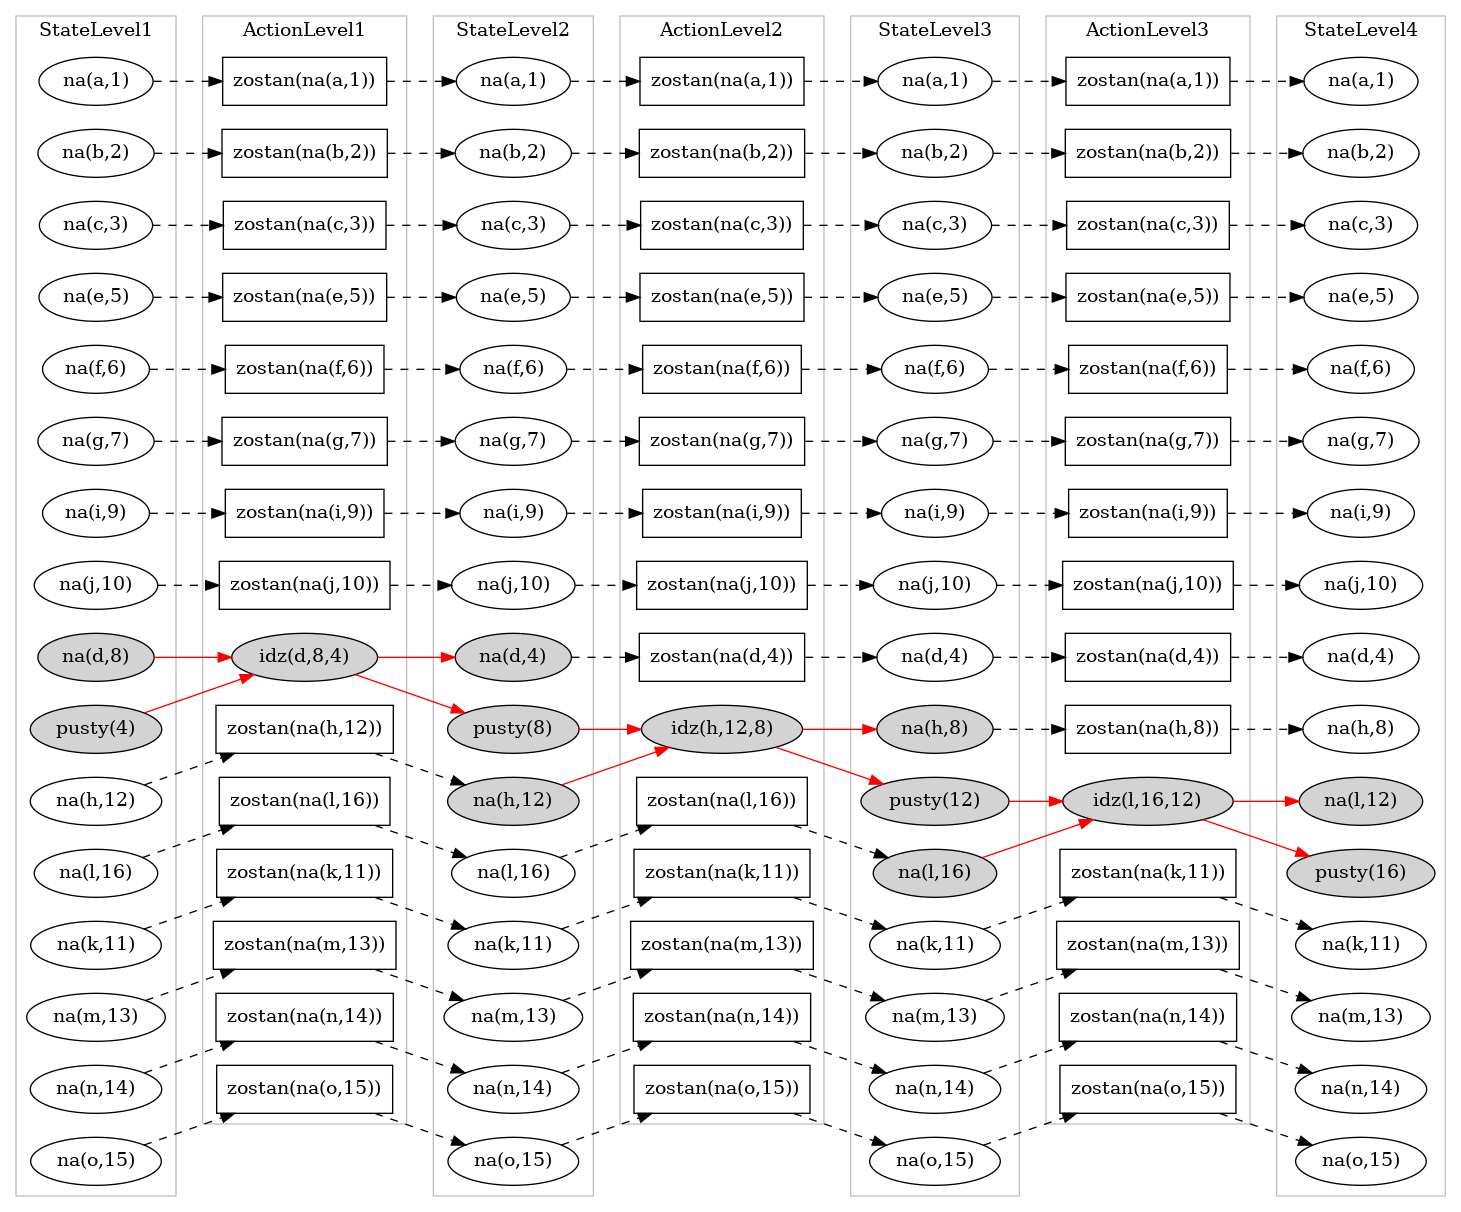
\includegraphics[scale=0.25]{15_graphplan}
            \centering
            \caption{Uproszczony graf planujący wygenerowany przez algorytm GRAPHPLAN przedstawiający stan każdego kafelka w danej warstwie. Węzły wypełnione 
            kolorem szarym obrazują stany, które są warunkami zajścia jak i efektami wykonywanej w danej warstwie akcji}
        \end{figure}

        \begin{figure}[H]
            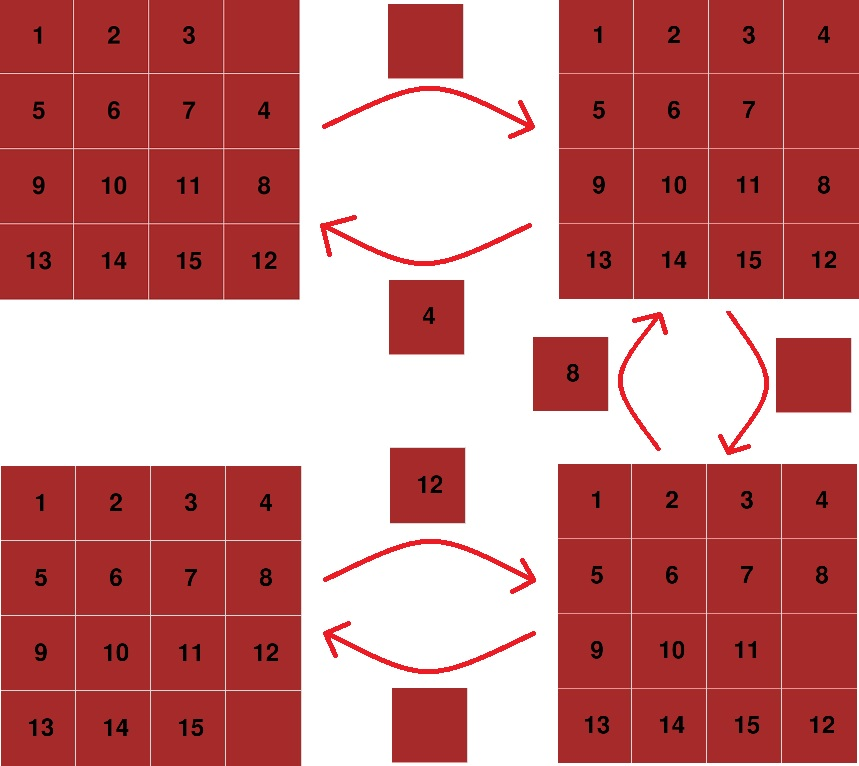
\includegraphics[scale=0.5]{15_zamiany}
            \centering
            \caption{Obrazowe rozwiązanie na podstawie wygenerowanego grafu}
        \end{figure}





    \subsection{Szczegóły implementacyjne}
    Ważnym jest, aby przedstawić omawiany świat zgodnie z wytycznymi ustalonymi przez język \textbf{STRIPS}. Z tego powodu należy dokładnie okreslić 
    każdą z istniejących w świecie relacji oraz poprawnie określić cel, jak i warunki początkowe.

    \subsection{Wyniki}

    \textbf{UWAGA:} Testy czasowe zaprezentowane w poniższych tabelach tyczą się osiągów samego algorytmu. Oznacza to, iż na czas wykonywania prób
    wyłączone zostały wszystkie poboczne funkcjonalności takie jak generowanie grafu, czy prezentowanie rozwiązania w formie graficznej. 
    Wykonanie poniższych badań w aplikacji może skutkować innymi wynikami, zwykle dłuższymi. Należy mieć to na uwadze przy potencjalnej 
    próbie odtwarzania badań.

    



    \subsection{Młodsza siostra- ósemka}

    \subsection{Wyniki dla 8}
    \subsection{Wnioski}
\section{CargoBot}
    \subsection{Wprowadzenie}
    \subsection{Przykład}
    \subsection{Szczegóły implementacyjne}
    \subsection{Wyniki}
    \subsection{Wnioski}
\section{Przemieszczanie w przestrzeni}
    \subsection{Wprowadzenie}
    \subsection{Przykład}
    \subsection{Szczegóły implementacyjne}
    \subsection{Wyniki}
    \subsection{Wnioski}
\section{Wieża Hanoi}
    \subsection{Wprowadzenie}
    \subsection{Przykład}
    \subsection{Szczegóły implementacyjne}
    \subsection{Wyniki}
    \subsection{Wnioski}
\section{Osiem Hetmanów}
    \subsection{Wprowadzenie}
    \subsection{Przykład}
    \subsection{Szczegóły implementacyjne}
    \subsection{Wyniki}
    \subsection{Wnioski}